% Options for packages loaded elsewhere
\PassOptionsToPackage{unicode}{hyperref}
\PassOptionsToPackage{hyphens}{url}
%
\documentclass[
]{book}
\usepackage{amsmath,amssymb}
\usepackage{lmodern}
\usepackage{iftex}
\ifPDFTeX
  \usepackage[T1]{fontenc}
  \usepackage[utf8]{inputenc}
  \usepackage{textcomp} % provide euro and other symbols
\else % if luatex or xetex
  \usepackage{unicode-math}
  \defaultfontfeatures{Scale=MatchLowercase}
  \defaultfontfeatures[\rmfamily]{Ligatures=TeX,Scale=1}
\fi
% Use upquote if available, for straight quotes in verbatim environments
\IfFileExists{upquote.sty}{\usepackage{upquote}}{}
\IfFileExists{microtype.sty}{% use microtype if available
  \usepackage[]{microtype}
  \UseMicrotypeSet[protrusion]{basicmath} % disable protrusion for tt fonts
}{}
\makeatletter
\@ifundefined{KOMAClassName}{% if non-KOMA class
  \IfFileExists{parskip.sty}{%
    \usepackage{parskip}
  }{% else
    \setlength{\parindent}{0pt}
    \setlength{\parskip}{6pt plus 2pt minus 1pt}}
}{% if KOMA class
  \KOMAoptions{parskip=half}}
\makeatother
\usepackage{xcolor}
\IfFileExists{xurl.sty}{\usepackage{xurl}}{} % add URL line breaks if available
\IfFileExists{bookmark.sty}{\usepackage{bookmark}}{\usepackage{hyperref}}
\hypersetup{
  pdftitle={Annalyse de données},
  pdfauthor={Abdoul Oudouss Diakite, Othmane ETTADLAOUI},
  hidelinks,
  pdfcreator={LaTeX via pandoc}}
\urlstyle{same} % disable monospaced font for URLs
\usepackage{color}
\usepackage{fancyvrb}
\newcommand{\VerbBar}{|}
\newcommand{\VERB}{\Verb[commandchars=\\\{\}]}
\DefineVerbatimEnvironment{Highlighting}{Verbatim}{commandchars=\\\{\}}
% Add ',fontsize=\small' for more characters per line
\usepackage{framed}
\definecolor{shadecolor}{RGB}{248,248,248}
\newenvironment{Shaded}{\begin{snugshade}}{\end{snugshade}}
\newcommand{\AlertTok}[1]{\textcolor[rgb]{0.94,0.16,0.16}{#1}}
\newcommand{\AnnotationTok}[1]{\textcolor[rgb]{0.56,0.35,0.01}{\textbf{\textit{#1}}}}
\newcommand{\AttributeTok}[1]{\textcolor[rgb]{0.77,0.63,0.00}{#1}}
\newcommand{\BaseNTok}[1]{\textcolor[rgb]{0.00,0.00,0.81}{#1}}
\newcommand{\BuiltInTok}[1]{#1}
\newcommand{\CharTok}[1]{\textcolor[rgb]{0.31,0.60,0.02}{#1}}
\newcommand{\CommentTok}[1]{\textcolor[rgb]{0.56,0.35,0.01}{\textit{#1}}}
\newcommand{\CommentVarTok}[1]{\textcolor[rgb]{0.56,0.35,0.01}{\textbf{\textit{#1}}}}
\newcommand{\ConstantTok}[1]{\textcolor[rgb]{0.00,0.00,0.00}{#1}}
\newcommand{\ControlFlowTok}[1]{\textcolor[rgb]{0.13,0.29,0.53}{\textbf{#1}}}
\newcommand{\DataTypeTok}[1]{\textcolor[rgb]{0.13,0.29,0.53}{#1}}
\newcommand{\DecValTok}[1]{\textcolor[rgb]{0.00,0.00,0.81}{#1}}
\newcommand{\DocumentationTok}[1]{\textcolor[rgb]{0.56,0.35,0.01}{\textbf{\textit{#1}}}}
\newcommand{\ErrorTok}[1]{\textcolor[rgb]{0.64,0.00,0.00}{\textbf{#1}}}
\newcommand{\ExtensionTok}[1]{#1}
\newcommand{\FloatTok}[1]{\textcolor[rgb]{0.00,0.00,0.81}{#1}}
\newcommand{\FunctionTok}[1]{\textcolor[rgb]{0.00,0.00,0.00}{#1}}
\newcommand{\ImportTok}[1]{#1}
\newcommand{\InformationTok}[1]{\textcolor[rgb]{0.56,0.35,0.01}{\textbf{\textit{#1}}}}
\newcommand{\KeywordTok}[1]{\textcolor[rgb]{0.13,0.29,0.53}{\textbf{#1}}}
\newcommand{\NormalTok}[1]{#1}
\newcommand{\OperatorTok}[1]{\textcolor[rgb]{0.81,0.36,0.00}{\textbf{#1}}}
\newcommand{\OtherTok}[1]{\textcolor[rgb]{0.56,0.35,0.01}{#1}}
\newcommand{\PreprocessorTok}[1]{\textcolor[rgb]{0.56,0.35,0.01}{\textit{#1}}}
\newcommand{\RegionMarkerTok}[1]{#1}
\newcommand{\SpecialCharTok}[1]{\textcolor[rgb]{0.00,0.00,0.00}{#1}}
\newcommand{\SpecialStringTok}[1]{\textcolor[rgb]{0.31,0.60,0.02}{#1}}
\newcommand{\StringTok}[1]{\textcolor[rgb]{0.31,0.60,0.02}{#1}}
\newcommand{\VariableTok}[1]{\textcolor[rgb]{0.00,0.00,0.00}{#1}}
\newcommand{\VerbatimStringTok}[1]{\textcolor[rgb]{0.31,0.60,0.02}{#1}}
\newcommand{\WarningTok}[1]{\textcolor[rgb]{0.56,0.35,0.01}{\textbf{\textit{#1}}}}
\usepackage{longtable,booktabs,array}
\usepackage{calc} % for calculating minipage widths
% Correct order of tables after \paragraph or \subparagraph
\usepackage{etoolbox}
\makeatletter
\patchcmd\longtable{\par}{\if@noskipsec\mbox{}\fi\par}{}{}
\makeatother
% Allow footnotes in longtable head/foot
\IfFileExists{footnotehyper.sty}{\usepackage{footnotehyper}}{\usepackage{footnote}}
\makesavenoteenv{longtable}
\usepackage{graphicx}
\makeatletter
\def\maxwidth{\ifdim\Gin@nat@width>\linewidth\linewidth\else\Gin@nat@width\fi}
\def\maxheight{\ifdim\Gin@nat@height>\textheight\textheight\else\Gin@nat@height\fi}
\makeatother
% Scale images if necessary, so that they will not overflow the page
% margins by default, and it is still possible to overwrite the defaults
% using explicit options in \includegraphics[width, height, ...]{}
\setkeys{Gin}{width=\maxwidth,height=\maxheight,keepaspectratio}
% Set default figure placement to htbp
\makeatletter
\def\fps@figure{htbp}
\makeatother
\setlength{\emergencystretch}{3em} % prevent overfull lines
\providecommand{\tightlist}{%
  \setlength{\itemsep}{0pt}\setlength{\parskip}{0pt}}
\setcounter{secnumdepth}{5}
\usepackage{booktabs}
\ifLuaTeX
  \usepackage{selnolig}  % disable illegal ligatures
\fi
\usepackage[]{natbib}
\bibliographystyle{plainnat}

\title{Annalyse de données}
\author{Abdoul Oudouss Diakite, Othmane ETTADLAOUI}
\date{30 May, 2022}

\begin{document}
\maketitle

{
\setcounter{tocdepth}{1}
\tableofcontents
}
\hypertarget{introduction}{%
\chapter*{Introduction}\label{introduction}}
\addcontentsline{toc}{chapter}{Introduction}

\hypertarget{linearModel}{%
\chapter{Régression linéaire}\label{linearModel}}

\hypertarget{introduction-1}{%
\section{Introduction}\label{introduction-1}}

La régression lineaire est une méthode statistique qui permet de trouver une relation lineaire entre des variables quantitives, une à expliquer et d'autres explicatives. C'est en fait un ajustement affine de la forme :

\begin{equation}
y_i = \beta_0 + \beta_1x_{i1} + \beta_2x_{i2} +\dots+\beta_px_{ip}+\epsilon_{i}\;\; 
\end{equation}

\[i\in\{1,2,3\dots,n\}\]

\begin{itemize}
\tightlist
\item
  \(y_i\) représentent la \(i\)ème valeur de la variable dépendantes \(y\).
\item
  \(x_{ij}\) représente la mesure de la \(i\)ème observation de la variable explicative \(X_j\)
\item
  les \(\beta_j\) sont les paramètres inconnus du modèle à estimer
\item
  \(\epsilon_i\) représente le bruit associé à la \(i\)ème observation\\
\end{itemize}

L'équation précédente peut être écrite sous une forme matricielle de cette manière :\\

\begin{equation}
y = X\beta +\epsilon
\end{equation}

avec :\\

\begin{equation}
y = \begin{pmatrix}y_1\\y_2\\\vdots\\y_n \end{pmatrix} \;\; 
X = \begin{pmatrix}
   1 & x_{11} & x_{12} & \dots &x_{1p}\\
   1 & x_{21} & x_{22} & \dots &x_{2p}\\
   \vdots &\vdots&\vdots & &\vdots\\
   1 & x_{n1} & x_{n2} & \dots &x_{np}
   \end{pmatrix} \;\;
\beta = \begin{pmatrix}\beta_0\\
   \beta_1\\
   \vdots\\
   \beta_n \end{pmatrix} \;\;
\epsilon = \begin{pmatrix}
   \epsilon_1\\
   \epsilon_2\\
   \vdots\\
   \epsilon_n \end{pmatrix} \;\;
\end{equation}

\hfill\break

Commençons par importer le jeu de données que nous nommerons \(dfcom\):\\

\begin{Shaded}
\begin{Highlighting}[]
\NormalTok{Communities }\OtherTok{=} \FunctionTok{read.csv}\NormalTok{(}\StringTok{"data/Communities.csv"}\NormalTok{,}\AttributeTok{row.names =} \DecValTok{1}\NormalTok{)}
\end{Highlighting}
\end{Shaded}

\begin{tabular}{l|l|l|l|r|r|r|r|r|r|r|r|r|r|r}
\hline
communityname & State & countyCode & communityCode & fold & pop & perHoush & pctBlack & pctWhite & pctAsian & pctHisp & pct12.21 & pct12.29 & pct16.24 & pct65up\\
\hline
BerkeleyHeightstownship & NJ & 39 & 5320 & 1 & 11980 & 3.10 & 1.37 & 91.78 & 6.50 & 1.88 & 12.47 & 21.44 & 10.93 & 11.33\\
\hline
Marpletownship & PA & 45 & 47616 & 1 & 23123 & 2.82 & 0.80 & 95.57 & 3.44 & 0.85 & 11.01 & 21.30 & 10.48 & 17.18\\
\hline
Tigardcity & OR & ? & ? & 1 & 29344 & 2.43 & 0.74 & 94.33 & 3.43 & 2.35 & 11.36 & 25.88 & 11.01 & 10.28\\
\hline
Gloversvillecity & NY & 35 & 29443 & 1 & 16656 & 2.40 & 1.70 & 97.35 & 0.50 & 0.70 & 12.55 & 25.20 & 12.19 & 17.57\\
\hline
Bemidjicity & MN & 7 & 5068 & 1 & 11245 & 2.76 & 0.53 & 89.16 & 1.17 & 0.52 & 24.46 & 40.53 & 28.69 & 12.65\\
\hline
Springfieldcity & MO & ? & ? & 1 & 140494 & 2.45 & 2.51 & 95.65 & 0.90 & 0.95 & 18.09 & 32.89 & 20.04 & 13.26\\
\hline
Norwoodtown & MA & 21 & 50250 & 1 & 28700 & 2.60 & 1.60 & 96.57 & 1.47 & 1.10 & 11.17 & 27.41 & 12.76 & 14.42\\
\hline
Andersoncity & IN & ? & ? & 1 & 59459 & 2.45 & 14.20 & 84.87 & 0.40 & 0.63 & 15.31 & 27.93 & 14.78 & 14.60\\
\hline
Fargocity & ND & 17 & 25700 & 1 & 74111 & 2.46 & 0.35 & 97.11 & 1.25 & 0.73 & 16.64 & 35.16 & 20.33 & 8.58\\
\hline
Wacocity & TX & ? & ? & 1 & 103590 & 2.62 & 23.14 & 67.60 & 0.92 & 16.35 & 19.88 & 34.55 & 21.62 & 13.12\\
\hline
\end{tabular}

\hypertarget{application-de-la-ruxe9gression-linuxe9aire-simple}{%
\section{Application de la régression linéaire simple}\label{application-de-la-ruxe9gression-linuxe9aire-simple}}

Comme nous l'avons mentionner dans l'introduction, le but de se projet est d'expliquer de différentes manières les meurtes aux USA. Par conséquent, on peut choisir comme variable dépendante, les crimes(\texttt{murders}) et chercher les variables explicatives. Dans le cas de le régression linéaire simple il doit exister une corrélation assez importante entre la variable \(y\)(\texttt{muders}) et \(X\) que nous recherchons actuellement. DOnc commençons par filtrer les fortes corrélation avec la variable \(y\) dans notre jeu de données.\\

\begin{Shaded}
\begin{Highlighting}[]
\CommentTok{\# Correlation matrix}
\NormalTok{corCom }\OtherTok{=}\NormalTok{ correlation}\SpecialCharTok{::}\FunctionTok{correlation}\NormalTok{(Communities)}
\CommentTok{\# Filtered correlation, bound =0.8}
\NormalTok{corCom[(corCom}\SpecialCharTok{$}\NormalTok{r}\SpecialCharTok{\textgreater{}}\FloatTok{0.8}\NormalTok{) }\SpecialCharTok{\&}\NormalTok{ corCom}\SpecialCharTok{$}\NormalTok{Parameter2}\SpecialCharTok{==}\StringTok{\textquotesingle{}murders\textquotesingle{}}\NormalTok{,]}
\end{Highlighting}
\end{Shaded}

\begin{verbatim}
## # Correlation Matrix (pearson-method)
## 
## Parameter1       | Parameter2 |    r |       95% CI | t(2213) |         p
## -------------------------------------------------------------------------
## pop              |    murders | 0.96 | [0.96, 0.96] |  159.80 | < .001***
## persUrban        |    murders | 0.96 | [0.95, 0.96] |  156.13 | < .001***
## persPoverty      |    murders | 0.98 | [0.97, 0.98] |  211.42 | < .001***
## kidsBornNevrMarr |    murders | 0.98 | [0.98, 0.98] |  221.27 | < .001***
## numForeignBorn   |    murders | 0.89 | [0.88, 0.90] |   92.94 | < .001***
## houseVacant      |    murders | 0.90 | [0.89, 0.90] |   95.29 | < .001***
## persEmergShelt   |    murders | 0.89 | [0.88, 0.90] |   93.14 | < .001***
## persHomeless     |    murders | 0.85 | [0.84, 0.86] |   76.49 | < .001***
## 
## p-value adjustment method: Holm (1979)
## Observations: 2215
\end{verbatim}

Le tableau précédent indique les variables fortement corrélées avec notre \(output\) \texttt{murders}. Prenons l'exemple de la variable \texttt{persPoverty} qui représente le nombre de personnes sous le seuil de pauvreté.\\

\begin{Shaded}
\begin{Highlighting}[]
\FunctionTok{library}\NormalTok{(ggplot2)}
\NormalTok{fig }\OtherTok{=} \FunctionTok{ggplot}\NormalTok{(}\AttributeTok{data =}\NormalTok{ Communities,}\FunctionTok{aes}\NormalTok{(}\AttributeTok{x=}\NormalTok{persPoverty,}\AttributeTok{y=}\NormalTok{murders))}\SpecialCharTok{+}
  \FunctionTok{geom\_point}\NormalTok{()}
\NormalTok{fig}
\end{Highlighting}
\end{Shaded}

\begin{center}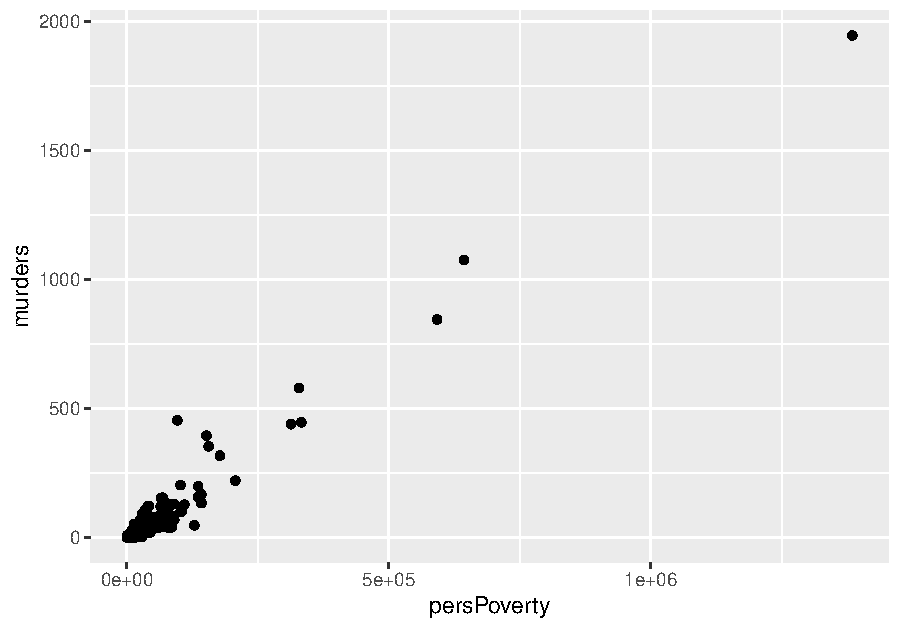
\includegraphics{_main_files/figure-latex/unnamed-chunk-4-1} \end{center}

La figure précédente laisse parraître qu'il pourrait effectivement exister une relation linéaire entre \texttt{murders} et \texttt{persPoverty}. Appliquons la fonction \texttt{lm()} pour voir ce qu'il en est vraiment ! Pour faire une analyse des résidus pltard, nous n'entrainerons que \(75\%\) du jeu de données et le reste servira à la prédiction.\\

\begin{Shaded}
\begin{Highlighting}[]
\FunctionTok{library}\NormalTok{(dplyr)}
\end{Highlighting}
\end{Shaded}

\begin{verbatim}
## 
## Attaching package: 'dplyr'
\end{verbatim}

\begin{verbatim}
## The following objects are masked from 'package:stats':
## 
##     filter, lag
\end{verbatim}

\begin{verbatim}
## The following objects are masked from 'package:base':
## 
##     intersect, setdiff, setequal, union
\end{verbatim}

\begin{Shaded}
\begin{Highlighting}[]
\CommentTok{\# Train\_Test\_Splite}
\FunctionTok{set.seed}\NormalTok{(}\DecValTok{1345}\NormalTok{)}
\CommentTok{\# Pourcentage de donnees correspondant a 25\%}
\NormalTok{per }\OtherTok{=} \FunctionTok{dim}\NormalTok{(Communities)[}\DecValTok{1}\NormalTok{]}\SpecialCharTok{\%/\%}\DecValTok{4}
\NormalTok{echantillon }\OtherTok{\textless{}{-}} \FunctionTok{sample}\NormalTok{(}\DecValTok{1}\SpecialCharTok{:}\FunctionTok{dim}\NormalTok{(Communities)[}\DecValTok{1}\NormalTok{]) }\SpecialCharTok{\%\textgreater{}\%}\NormalTok{ .[}\DecValTok{1}\SpecialCharTok{:}\NormalTok{per]}
\NormalTok{lmDataTrain }\OtherTok{=}\NormalTok{ Communities[}\SpecialCharTok{{-}}\NormalTok{echantillon,}\FunctionTok{c}\NormalTok{(}\StringTok{"murders"}\NormalTok{,}\StringTok{"persPoverty"}\NormalTok{)]}
\NormalTok{lmDataTest }\OtherTok{=}\NormalTok{ Communities[echantillon,}\FunctionTok{c}\NormalTok{(}\StringTok{"murders"}\NormalTok{,}\StringTok{"persPoverty"}\NormalTok{)]}
\end{Highlighting}
\end{Shaded}

\begin{Shaded}
\begin{Highlighting}[]
\CommentTok{\#Model Training}
\NormalTok{lmSimple }\OtherTok{\textless{}{-}} \FunctionTok{lm}\NormalTok{(murders}\SpecialCharTok{\textasciitilde{}}\NormalTok{persPoverty,}\AttributeTok{data =}\NormalTok{ lmDataTrain)}
\FunctionTok{summary}\NormalTok{(lmSimple)}
\end{Highlighting}
\end{Shaded}

\begin{verbatim}
## 
## Call:
## lm(formula = murders ~ persPoverty, data = lmDataTrain)
## 
## Residuals:
##     Min      1Q  Median      3Q     Max 
## -136.43   -1.13    1.32    2.52  317.80 
## 
## Coefficients:
##               Estimate Std. Error t value Pr(>|t|)    
## (Intercept) -3.271e+00  3.340e-01  -9.796   <2e-16 ***
## persPoverty  1.449e-03  7.447e-06 194.519   <2e-16 ***
## ---
## Signif. codes:  0 '***' 0.001 '**' 0.01 '*' 0.05 '.' 0.1 ' ' 1
## 
## Residual standard error: 13.4 on 1660 degrees of freedom
## Multiple R-squared:  0.958,  Adjusted R-squared:  0.9579 
## F-statistic: 3.784e+04 on 1 and 1660 DF,  p-value: < 2.2e-16
\end{verbatim}

La sortie de la fonction \texttt{summary()} indique des \(p-values\) très inférieures à \(5\%\), donc on rejette l'hypothèse de nullité des \(\beta\). On peut aussi constater que le coefficient de détermination \(R^2\) vaut \(0.958\) ce qui signifie que notre modèle a un score de \(95.8\%\). Ce dernier reflète une bonne qualité du modèle.\\

\begin{Shaded}
\begin{Highlighting}[]
\NormalTok{ggstatsplot}\SpecialCharTok{::}\FunctionTok{ggscatterstats}\NormalTok{(}
  \AttributeTok{data =}\NormalTok{ lmDataTrain, }
  \AttributeTok{x =}\NormalTok{ persPoverty, }
  \AttributeTok{y =}\NormalTok{ murders,}
  \AttributeTok{xlab  =} \StringTok{"le nombre de personnes sous le seuil de pauvreté"}\NormalTok{,}
  \AttributeTok{ylab  =} \StringTok{"le nombre de meurtres"}\NormalTok{,}
  \AttributeTok{title =} \StringTok{"Droite de régression"}\NormalTok{,}
  \AttributeTok{messages =} \ConstantTok{FALSE}
\NormalTok{)}
\end{Highlighting}
\end{Shaded}

\begin{verbatim}
## Registered S3 method overwritten by 'ggside':
##   method from   
##   +.gg   ggplot2
\end{verbatim}

\begin{verbatim}
## `stat_bin()` using `bins = 30`. Pick better value with `binwidth`.
## `stat_bin()` using `bins = 30`. Pick better value with `binwidth`.
\end{verbatim}

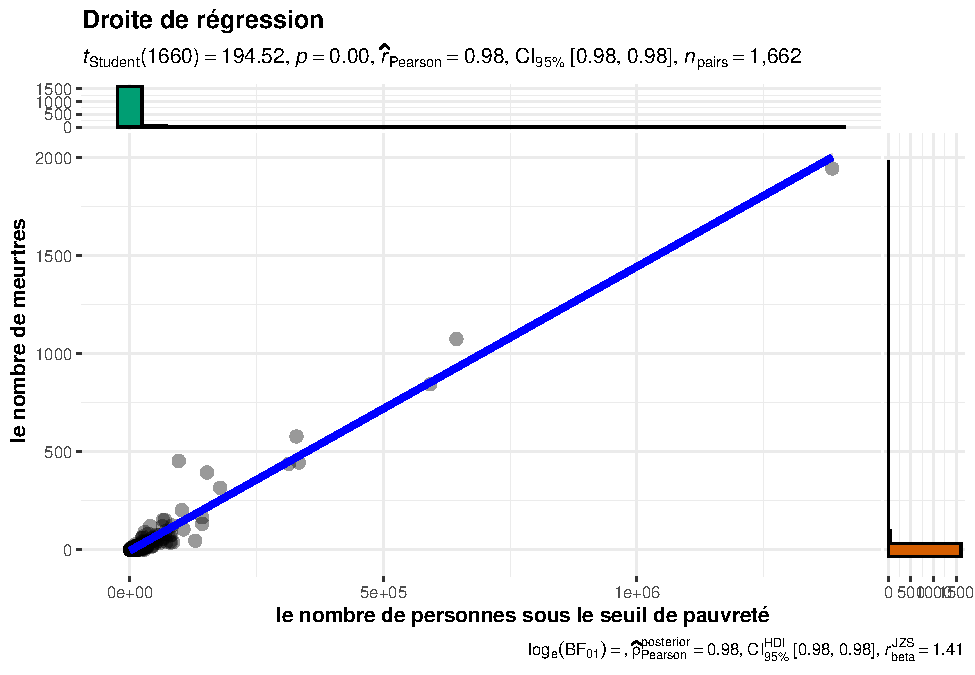
\includegraphics{_main_files/figure-latex/unnamed-chunk-7-1.pdf}

A présent, nous pouvons utiliser notre échantillon non entrainé de données pour prédire à partir de notre model, quel aurait était le nombre de meurtres pour chauque \(x_i\).\\

\begin{Shaded}
\begin{Highlighting}[]
\NormalTok{X\_test}\OtherTok{=}\FunctionTok{as.data.frame}\NormalTok{(lmDataTest[[}\StringTok{"persPoverty"}\NormalTok{]])}
\FunctionTok{colnames}\NormalTok{(X\_test)}\OtherTok{=}\StringTok{"persPoverty"}
\NormalTok{y\_predict }\OtherTok{=} \FunctionTok{predict}\NormalTok{(}\AttributeTok{object =}\NormalTok{ lmSimple,X\_test)}
\end{Highlighting}
\end{Shaded}

On peut représenter le graphe des \(\hat y\) prédits et des \(y\). Pour un modèle parfait, le nuage de point doit être sur la première bissectrice.\\

\begin{Shaded}
\begin{Highlighting}[]
\FunctionTok{ggplot}\NormalTok{(}\AttributeTok{data =}\NormalTok{lmDataTest) }\SpecialCharTok{+}
  \FunctionTok{geom\_point}\NormalTok{(}\FunctionTok{aes}\NormalTok{(persPoverty,murders),}\AttributeTok{color =} \StringTok{\textquotesingle{}darkgreen\textquotesingle{}}\NormalTok{,}
             \AttributeTok{size =}\DecValTok{2}\NormalTok{,}\AttributeTok{shape=}\DecValTok{22}\NormalTok{,}\AttributeTok{fill =}\StringTok{"darkgreen"}\NormalTok{) }\SpecialCharTok{+}
  \FunctionTok{geom\_point}\NormalTok{(}\FunctionTok{aes}\NormalTok{(}\AttributeTok{x =}\NormalTok{ persPoverty, }\AttributeTok{y =}\NormalTok{y\_predict), }\AttributeTok{color =}\StringTok{\textquotesingle{}blue\textquotesingle{}}\NormalTok{) }\SpecialCharTok{+}
  \FunctionTok{geom\_segment}\NormalTok{(}\FunctionTok{aes}\NormalTok{(}\AttributeTok{x =}\NormalTok{persPoverty , }
                   \AttributeTok{y =}\NormalTok{ murders, }\AttributeTok{xend =}\NormalTok{ persPoverty, }\AttributeTok{yend =}\NormalTok{ y\_predict),}
               \AttributeTok{color =} \StringTok{\textquotesingle{}red\textquotesingle{}}\NormalTok{)}
\end{Highlighting}
\end{Shaded}

\begin{figure}

{\centering 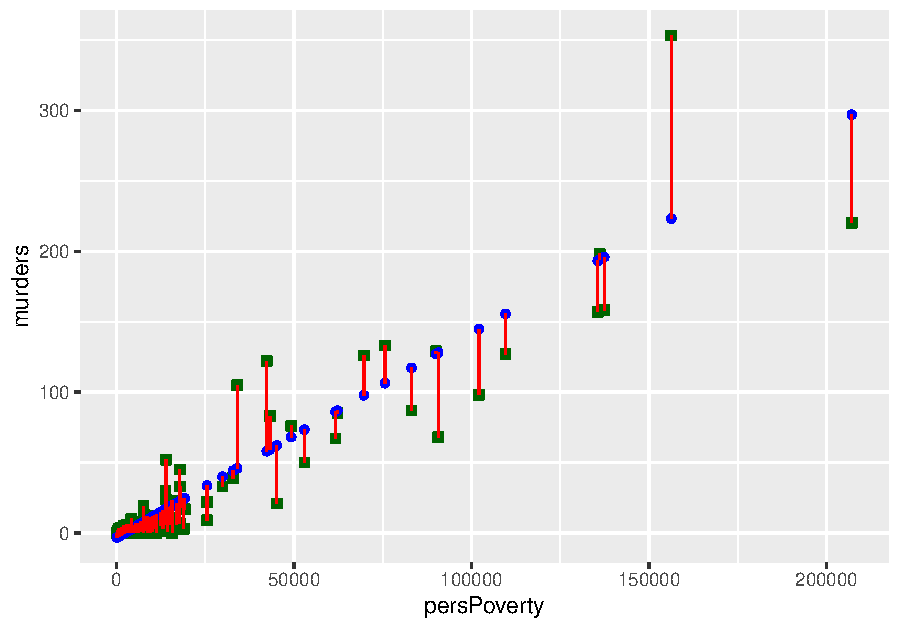
\includegraphics{_main_files/figure-latex/unnamed-chunk-9-1} 

}

\caption{Les segments en rouges représentent les résidus, les carrés verts les y non entrainés qui ont servi au test et les points bleus représentent les y prédits à partir de notre modèle.}\label{fig:unnamed-chunk-9}
\end{figure}

On peut aussi visualiser la répartition des résidus du modèle \texttt{lmSimple} autour de leur moyenne \(0\).\\

\begin{Shaded}
\begin{Highlighting}[]
\FunctionTok{plot}\NormalTok{(lmSimple}\SpecialCharTok{$}\NormalTok{residuals)}
\end{Highlighting}
\end{Shaded}

\begin{figure}

{\centering 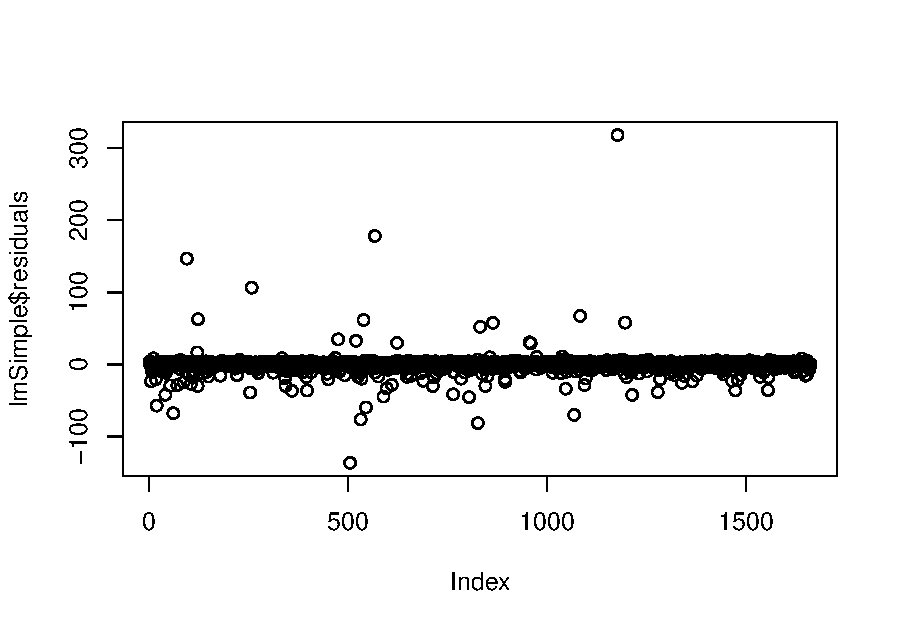
\includegraphics{_main_files/figure-latex/unnamed-chunk-10-1} 

}

\caption{On constate une répartition des résidus autour de 0}\label{fig:unnamed-chunk-10}
\end{figure}

  \bibliography{book.bib,packages.bib}

\end{document}
